<<<<<<< HEAD
\begin{name}
	{\tenchude}
	{TOÁN 10}
	{LỚP TOÁN THẦY PHÁT}
	{{Học tập không phải là dồn ép tất cả mọi thứ vào đầu.\\ Biết cách học vừa đủ, đó mới là người thông minh}}
\end{name}
\TN
\begin{ex}%[0-HK1-CT-6-HungVuong-HCM-2324]%[VN-MT-6, Nguyễn Hữu Đức]%[0D6N3-3]
Một nhóm có $10$ học sinh tham gia một kỳ thi. Số điểm thi của $10$ học sinh đó (thang điểm $10$) được sắp xếp từ thấp đến cao như sau:
\begin{center}
$\begin{array}{cccccccccc}
$0$&$1$&$2$&$4$&$4$&$5$&$7$&$8$&$8$&$9$.
\end{array}$
\end{center}
Khi đó, trung vị của mẫu số liệu trên là
\choice
{$5$}
{$4$}
{\True $4{,}5$}
{$5{,}5$}
\loigiai{
Sắp xếp mẫu số liệu theo thứ tự không giảm ta được
\begin{center}
$\begin{array}{cccccccccc}
$0$&$1$&$2$&$4$&$4$&$5$&$7$&$8$&$8$&$9$.
\end{array}$
\end{center}
Số liệu có $10$ phần tử nên trung vị là $M_e=\dfrac{4+5}{2}=4{,}5$.
}
\end{ex}

\begin{ex}%[0-HK1-CT-1-BuiThiXuan-TPHCM-2324]%[VN-MT-6, VM013]%[0D6N4-2]
Mẫu số liệu thống kê tổng số giờ nắng trong năm $2019$ theo từng tháng được đo bởi trạm quan sát khí tượng ở Tuyên Quang:
\begin{center}
\begin{tabular}{cccccccccccc}
$25$ & $89$ & $72$ & $117$ & $106$ & $177$ & $156$ & $203$ & $227$ & $146$ & $117$ & $145$ \\
\end{tabular}
\end{center}
Hãy xác định khoảng biến thiên của số giờ nắng ở Tuyên Quang trong năm $2019$
\choice
{$227$}
{$145$}
{\True $202$}
{$120$}
\loigiai
{
Khoảng biến thiên số giờ nắng ở Tuyên Quang trong năm $2019$ là $R=227-25=202$.
}
\end{ex}

\begin{ex}%[0D8H1-3]%[TeX Hoá Đề CK2 - Form 2025 - Đợt 2 - GV: Võ Thị Thùy Trang]
Từ thành phố $A$ đến thành phố $B$ có $3$ con đường, từ thành phố $A$ đến thành phố $C$ có $2$ con đường, từ thành phố $B$ đến thành phố $D$ có $2$ con đường, từ thành phố $C$ đến thành phố $D$ có $3$ con đường, không có con đường nào nối từ thành phố $C$ đến thành phố $B$. Hỏi có bao nhiêu con đường đi từ thành phố $A$ đến thành phố $D$.
\choice
{$6$}
{\True $12$}
{$18$}
{$36$}
\loigiai{\immini
{Số cách đi từ $A$ đến $D$ bằng cách đi từ $A$ đến $B$ rồi đến $D$ là $3\cdot 2=6$.\\
Số cách đi từ $A$ đến $D$ bằng cách đi từ $A$ đến $C$ rồi đến $D$ là $2\cdot 3=6$.\\
Vậy có $6+6=12$ cách.}
{\begin{tikzpicture}[scale=.75, dot/.style = {circle, fill, minimum size=#1,
inner sep=0pt, outer sep=0pt}, dot/.default = 6pt,
nodes = {font=\sffamily}]
\coordinate[label=left:$A$] (A) at (0,0);
\coordinate[label=above:$B$] (B) at (2,2.5);
\coordinate[label=right:$C$] (C) at (3,0);
\coordinate[label=above:$D$] (D) at ($(B)+(C)-(A)$);
\draw
(A)--(B)node[pos=0.5,black,left]{$3$}
(D)--(B)node[pos=0.5,sloped,black,above]{$2$}
(C)--(D)node[pos=0.5,black,right]{$3$}
(A)--(C)node[pos=0.5,sloped,black,below]{$2$}	;
\foreach \diem in {A,B,C,D} \fill[black](\diem)circle(1.5pt);
\end{tikzpicture}}
}
\end{ex}

\begin{ex}%[0D8H2-3]
Từ các chữ số $0$; $1$; $2$; $3$; $4$; $5$; $6$. Có thể lập được bao nhiêu số có 4 chữ số, các chữ số đôi một khác nhau?
\choice
{$35$}
{$840$}
{$70$}
{\True$720$}
\loigiai{
Gọi số có 4 chữ số khác nhau được lập từ các số đã cho là $\overline{abcd}$ ($a\neq 0$).\\
Vì $a\neq 0$ nên có $6$ cách chọn $a$\\
Với mỗi cách chọn $a$ có $\mathrm{A}^6_3$ cách chọn $b$, $c$, $d$.\\
Như vậy có tất cả $6\cdot\mathrm{A}^6_3=720$ số.
}
\end{ex}

\begin{ex}%[BG - 10 New - 4in1,Phan Chiến Thắng]%[0D8H2-4]
Có bao nhiêu khả năng có thể xảy ra đối với thứ tự giữa các đội trong một giải bóng có $5$ đội bóng? (Giả sử rằng không có hai đội nào có điểm trùng nhau).
\choice
{$100$}
{$60$}
{\True $120$}
{$80$}
\loigiai{
Số các khả năng có thể xảy ra đối với thứ tự giữa các đội trong một giải bóng có $5$ đội bóng là số hoán vị của $5$ phần tử nên có $5!=120$ cách.
}
\end{ex}

\begin{ex}%[0D8H2-6]
Trong mặt phẳng cho một tập hợp gồm $ 6 $ điểm phân biệt. Có bao nhiêu véc-tơ khác véc-tơ $ \overrightarrow{0} $ có điểm đầu và điểm cuối thuộc tập hợp điểm này?
\choice
{$ 15 $}
{$ 12 $}
{$ 1440 $}
{\True $ 30 $}
\loigiai{
Mỗi cặp sắp thứ tự gồm hai điểm $ (A, B) $ cho ta một véc-tơ có điểm đầu $ A $ và điểm cuối $ B $ và ngược lại. Như vậy, mỗi véc-tơ có thể xem là một chỉnh hợp chập $ 2 $ của tập hợp $ 6 $ điểm đã cho. Suy ra có $ \mathrm{A}_6^2=30 $ cách.
}
\end{ex}

\begin{ex}%[BG - 10 New - 4in1,Phú Thạch]%[0D8H3-2]
Trong khai triển $(2 a-b)^5$, hệ số của số hạng thứ $3$ bằng
\choice
{$-80$}
{\True $80$}
{$-10$}
{$10$}
\loigiai
{Ta có $(2 a-b)^5=\mathrm{C}_5^0\cdot \left(2a\right)^5(-b)^0+\mathrm{C}_5^1\cdot \left(2a\right)^4(-b)^1+\mathrm{C}_5^2\cdot \left(2a\right)^3(-b)^2+\mathrm{C}_5^4\cdot \left(2a\right)^2(-b)^3+\cdots$\\
Số hạng thứ $3$ trong khai triển $(2 a-b)^5$ là $\mathrm{C}_5^2\cdot \left(2a\right)^3(-b)^2$.\\
Suy ra hệ số của số hạng thứ $3$ trong khai triển $(2 a-b)^5$ bằng $80$.

}
\end{ex}

\begin{ex}%[0-HK1-KN-8-TranHungDao-HaNoi-2324]%[VN-MT-6,Nguyễn Kiều Nhã Tú]%[0H9H1-2]
Cho $\overrightarrow{a}=(-1;2)$, $\overrightarrow{b}=(5;-7)$. Tọa độ vectơ $\overrightarrow{b}-\overrightarrow{a}$ là
\choice
{$(-6;9)$}
{$(-5;-14)$}
{$(4;-5)$}
{\True $(6;-9)$}
\loigiai{
Ta có $\overrightarrow{b}-\overrightarrow{a}=\left(5-(-1);-7-2\right)=(6;-9)$.
}
\end{ex}

\begin{ex} %[0H9H3-2]
Đường thẳng đi qua hai điểm $M(-1 ; 2), N(3 ; 1)$ có phương trình tổng quát là
\choice
{$4 x-y-6=0$}
{$2 x+3 y-9=0$}
{$x-4 y+9=0$}
{\True $x+4 y-7=0$}
\loigiai{
Đường thẳng đi qua hai điểm $M(-1 ; 2), N(3 ; 1)$ có véc-tơ chỉ phương là $\vec{MN}=(4;-1)$ nên nó có một véc-tơ pháp tuyến là $\vec{n}=(1;4)$.\\
Phương trình tổng quát của đường thẳng $MN$ có dạng
\[(x+1)+4(y-2)=0\Leftrightarrow x+4y-7=0.\]
}
\end{ex}

\begin{ex}%[0H9H4-2]%[Dự án GHKII - K10-11 - PNL - NH23-24]%[Thanh Thủy]
Phương trình nào là phương trình của đường tròn tâm $I(-3;4)$, có bán kính $R=2$?
\choice
{$\left(x-3\right)^2+\left(y-4\right)^2=4$}
{\True $\left(x+3\right)^2+\left(y-4\right)^2=4$}
{$\left(x+3\right)^2+\left(y+4\right)^2=4$}
{$\left(x+3\right)^2+\left(y-4\right)^2=2$}
\loigiai
{
Phương trình của đường tròn tâm $I(-3;4)$, có bán kính $R=2$ là $\left(x+3\right)^2+\left(y-4\right)^2=4$.
}
\end{ex}

\begin{ex}%[0H9H5-2]
Phương trình chính tắc của elip $(E)$ có tiêu cự bằng $6$ và đi qua điểm $A(5;0)$ là
\choice
{$\dfrac{x^2}{100}+\dfrac{y^2}{81}=1$}
{$\dfrac{x^2}{15}+\dfrac{y^2}{16}=1$}
{$\dfrac{x^2}{25}+\dfrac{y^2}{9}=1$}
{\True $\dfrac{x^2}{25}+\dfrac{y^2}{16}=1$}
\loigiai{
Do $(E)$ có tiêu cự bằng $6$ nên $2c=6 \Rightarrow c=3$.\\
Do $(E)$ đi qua điểm $A(5;0)$ nên $a=5 \Rightarrow b^2=a^2-c^2=25-9=16$.\\
Phương trình chính tắc của $(E)$ là $(E)\colon \dfrac{x^2}{25}+\dfrac{y^2}{16}=1$.
}
\end{ex}

\begin{ex}%[0H9H5-4]
Tâm sai của Hyperbol $\dfrac{x^{2}}{5} -\dfrac{y^{2}}{4} =1$ bằng
\choice{$\dfrac{\sqrt{5}}{5}$}
{\True $\dfrac{3}{\sqrt{5}}$}
{$\dfrac{3}{5}$}
{$\dfrac{4}{5}$}
\loigiai{
Ta có $a^{2} =5; b^{2} =4$ suy ra $\heva{c^{2} &=5+4=9 \\ a&=\sqrt{5}} \Rightarrow c=3 $. Tâm sai của Hyperbol là $e=\dfrac{c}{a} =\dfrac{3}{\sqrt{5}}$.
}
\end{ex}
\TNTF
\begin{ex}%[BG - 10 New - 4in1,Phan Chiến Thắng]%[0D8H2-4]
Có $5$ nam sinh và $3$ nữ sinh được sắp xếp vào một hàng dọc.
\choiceTF[t]
{\True Số cách sắp xếp $8$ học sinh vào một hàng dọc là $40320$}
{Số cách sắp xếp $8$ bạn học sinh sao cho có một bạn nam đứng đầu hàng là $720$}
{\True Số cách sắp xếp $8$ bạn học sinh sao cho học sinh cùng giới đứng cạnh nhau là $1440$}
{\True Số cách sắp xếp $8$ bạn học sinh sao cho học sinh nữ luôn đứng cạnh nhau là $4320$}
\loigiai{
\begin{itemchoice}
\itemch Đúng. Số cách sắp xếp là $8!=40320$.
\itemch Sai. Số cách sắp xếp là $5\cdot 7!=25200$.
\itemch Đúng. Số cách sắp xếp $8$ bạn học sinh sao cho học sinh cùng giới đứng cạnh nhau là $2\cdot 5!\cdot 3!=1440$
\itemch Đúng. Số cách sắp xếp $8$ bạn học sinh sao cho học sinh nữ luôn đứng cạnh nhau là $4320$.
\end{itemchoice}
}
\end{ex}

\begin{ex}%[Dự án 18 - TeamTeXHoa - Phạm Quốc Toàn]%[0H9H4-5]
Trong hệ trục tọa độ $Oxy$, cho đường tròn $\left(C \right)$ tâm $I \left(1;2 \right)$ và cắt đường thẳng $\Delta\colon 3x+4y-6=0$ tại hai điểm $A$, $B$ sao cho $AB=4$. Trong mỗi ý a), b), c), d) sau, hãy chọn đúng hoặc sai.
\choiceTF
{Khoảng cách từ tâm $I$ đến đường thẳng $\Delta$ bằng $2$}
{\True Bán kính đường tròn bằng $\sqrt{5}$}
{\True Phương trình đường tròn $\left(C \right) \colon x^2+y^2-2x-4y=0$}
{Điểm $M \left(3;1 \right)$ nằm trong đường tròn $\left(C \right)$}
\loigiai{
\begin{center}
\begin{tikzpicture}[>=stealth, x=1.0 cm, y=1.0 cm]
% \draw[->] (-4,0) --(0,0) node[below left]{$O$} -- (4,0) node[below]{$x$};
% \draw[->](0,-4)--(0, 4) node[right]{$y$};
\draw(0,0) circle (3); %(0,0) là tọa độ tâm, 1 là bán kính
\draw(-4,2) -- (4,2) (0, 0) -- (0, 2);
\draw (0,0) circle (1pt) node[below]{$I$};
\draw (0,2) circle (1pt) node[above]{$H$};
\draw (3.5,2) circle node[below]{$\Delta$};
\draw (-2.24,2) circle (1pt) node[above left]{$A$};
\draw (2.24,2) circle (1pt) node[above right]{$B$};
\draw (-2,-2.24) circle (1pt) node[below left]{$M$};
\end{tikzpicture}
\end{center}
\begin{itemchoice}
\itemch Kẻ $IH \perp \Delta$. \\
Ta có $IH=d_{\left(I, \Delta\right)}=\dfrac{\left| 3+8-6\right|}{\sqrt{3^2+4^2}}=1$.
\itemch $IH \perp AB \Rightarrow H$ là trung điểm $AB$ và $AH=2$. \\
$R=IA=\sqrt{IH^2+AH^2}=\sqrt{1^2+2^2}=\sqrt{5}$.
\itemch Phương trình đường tròn $ \left(C \right)$ tâm $I \left(1;2 \right)$, bán kính $R=\sqrt{5}$ là $\left(C \right) \colon \left(x-1 \right)^2+ \left(y-2 \right)^2=5$ hay $\left(C \right) \colon x^2+y^2-2x-4y=0$.
\itemch Ta có $\overrightarrow{IM}= \left(2;-1 \right) \Rightarrow IM=\sqrt{2^2+ \left(-1 \right)^2}=\sqrt{5}=R$. Suy ra $M\in \left(C \right)$.
\end{itemchoice}
}
\end{ex}
\TNSA
\begin{ex}%[Dự án đề theo cấu trúc mới 2025-NCT]%[0D0V2-5]
Một lô hàng có $14$ sản phẩm, trong đó có đúng $2$ phế phẩm. Lấy ngẫu nhiên $8$ sản phẩm từ lô hàng đó. Tính xác suất biến cố $A$ \lq\lq Trong $8$ sản phẩm lấy ra có không quá $1$ phế phẩm\rq\rq.
\shortans{$0,69$}
\loigiai{
Số cách lấy ngẫu nhiên $8$ sản phẩm từ lô hàng là $ n(\Omega)=\mathrm{C}_{14}^8=3003$.\\
Số cách lấy ngẫu nhiên $8$ sản phẩm mà không có phế phẩm là $ \mathrm{C}_{12}^8=495$\\
Số cách lấy ngẫu nhiên $8$ sản phẩm mà trong đó có đúng 1 phế phẩm là $ \mathrm{C}_2^1\cdot \mathrm{C}_{12}^7=1584$.\\
Khi đó số phần tử của biến cố $A$ “Trong $8$ sản phẩm lấy ra có không quá $1$ phế phẩm” là $ n(A)=495+1584=2079$.\\
Khi đó xác suất biến cố $A$ là $P\left( A \right)=\dfrac {n\left( A \right)}{n( \Omega )}=\dfrac {2079}{3003}=\dfrac {9}{13}\approx 0{,}69$.
}
\end{ex}

\begin{ex}%[24-25 giảng K10 - K11, Phan Quốc Trí]%[0D8H2-5]
Một người nông dân có $ 10 $ cây giống khác nhau gồm $ 6 $ cây xoài và $ 4 $ cây mít. Người ấy muốn chọn $ 4 $ cây để trồng sao cho phải có đủ $ 2 $ loại xoài và mít. Hỏi người ấy có bao nhiêu cách để chọn?
\shortans[oly]{194}
\loigiai{
Ta có  các trường hợp như sau:
\begin{itemize}
\item TH1: $ 1 $ cây xoài và $ 3 $ cây mít.\\
Số cách chọn $ 1 $ trong $ 6 $ cây xoài là $ 6 $ cách.\\
Số cách chọn $ 3 $ trong $ 4 $ cây mít là $ \mathrm{C}_4^3=4 $ cách.\\
Suy ra TH1 có $ 6\times4=24 $ cách.
\item TH2: $ 2 $ cây xoài và $ 2 $ cây mít.\\
Tương tự, ta có: $ \mathrm{C}_6^2\times\mathrm{C}_4^2=90 $ cách.
\item TH3: $ 3 $ cây xoài và $ 1 $ cây mít.\\
Tương tự, ta có: $ \mathrm{C}_6^3\times4=80 $ cách.
\end{itemize}
Vậy số cách chọn theo yêu cầu bài toán là $ 24+90+80=194 $ cách.
}
\end{ex}

\begin{ex}%[Đề chuẩn hóa Toán 11]%[Nguyễn Trung Kiên]%[0D8H3-4]
Hệ số của số hạng chứa $x^5$ trong khai triển $(2x+1)(x-3)^5$ là bao nhiêu?
\shortans{$-29$}
\loigiai{
Ta có
\allowdisplaybreaks
\begin{eqnarray*}
(x-3)^5&=& x^5 + 5x^4\cdot (-3)^1 + 10x^3\cdot (-3)^2 + 10x^2\cdot (-3)^3 + 5x\cdot (-3)^4 + (-3)^5\\
&=& x^5 - 15x^4 + 90x^3 - 270x^2 + 405x - 243.
\end{eqnarray*}
Suy ra
\begin{eqnarray*}
(2x+1)(x-3)^5&=& (2x+1)\left(x^5 - 15x^4 + 90x^3 - 270x^2 + 405x - 243\right)\\
&=& 2x^6 - 29x^5 + 165x^4 - 450x^3 + 540x^2 - 81x - 243.
\end{eqnarray*}
Vậy số hạng chứa $x^5$ trong khai triển là $-29$.
}
\end{ex}

\begin{ex}%[0H9V4-7]
Một kiến trúc sư muốn thiết kế một khung cửa sổ hình chữ nhật lắp vào một ô tròn trên tường có bán kính $4$ mét. Kiến trúc sư muốn cửa sổ có kích thước lớn nhất để đón ánh sáng vào căn phòng. Hỏi diện tích lớn nhất của cửa sổ có thể đạt được là bao nhiêu?
\shortans{32}
\loigiai{
\immini[thm]{
Đặt trục tọa độ sao cho tâm đường tròn (tâm hình chữ nhật) trùng gốc tọa độ và điểm $(x; y)$ như hình vẽ.\\
Ta có phương trình đường tròn $(C)\colon x^2 + y^2 = 16$ hay $y = \pm\sqrt{16-x^2}$.\\
Khi đó chiều dài của số hình chữ nhật là $2x$, chiều rộng là $2y$, với $x>0$, $y>0$ nằm trên đường tròn $(C)$.\\
Diện tích cửa sổ hình chữ nhật là $S = 2x \cdot 2y = 4xy = 4x\sqrt{16-x^2}$.\\
Xét hàm số $S(x) = 4x\sqrt{16-x^2}$ với $0\leq x\leq 4$.\\
Ta có $S'(x) = 4\sqrt{16-x^2} - \dfrac{4x^2}{\sqrt{16-x^2}} = \dfrac{64 - 8x^2}{\sqrt{16-x^2}}$.\\
Cho $S'(x) = 0 \Leftrightarrow 64 - 8x^2 = 0 \Leftrightarrow \hoac{&x = 2\sqrt{2} \\& x = -2\sqrt{2} \text{ (loại)}.}$
}{
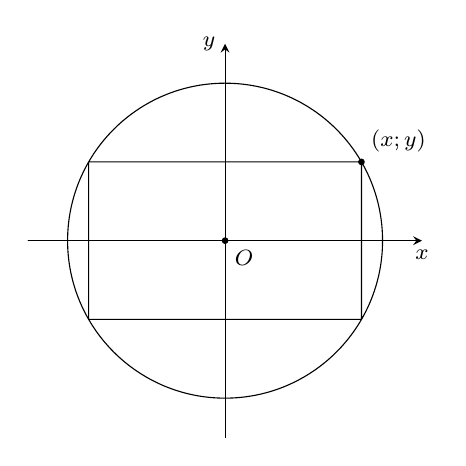
\begin{tikzpicture}[scale=1, font=\footnotesize, line cap=round, line join=round, >=stealth]
\def\r{2}
\path (0,0)coordinate(O)+(30:\r)coordinate(A)+(150:\r)coordinate(B)+(210:\r)coordinate(C)+(-30:\r)coordinate(D);
\draw[->] (-\r-.5,0)--(\r+.5,0)node[below]{$x$};
\draw[->] (0,-\r-.5)--(0,\r+.5)node[left]{$y$};
\draw (O)circle(\r cm) (A)--(B)--(C)--(D)--cycle;
\draw[fill=black] (0,0)node[below right]{$O$}circle(1pt) (A)node[above right]{$(x;y)$}circle(1pt);
\end{tikzpicture}
}
\noindent
Ta có $S(0) = 0$; $S(4) = 0$; $S(2\sqrt{2}) = 32$.\\
Vậy cửa sổ hình chữ nhật lớn nhất nội tiếp đường tròn có bán kính $4$ sẽ là hình vuông với diện tích $32$, chiều dài và chiều rộng bằng $2\sqrt{2} \cdot 2 = 4\sqrt{2}$ (từ $2x$ và $2y$ với $x=y=2\sqrt{2}$).
}
\end{ex}
\TL
\begin{ex}%[0D8H3-2]%[Dự án tex đề CKII - Đợt 15]%[Đình Trí]
Tìm hệ số chứa $ x^4 $ trong khai triển $ (2x-1)^5 $.
\loigiai
{
Ta có
\begin{eqnarray*}
(2x-1)^5 &=&\mathrm{C}_5^0(2x)^5-\mathrm{C}_5^1(2x)^4+\mathrm{C}_5^2(2x)^3-\mathrm{C}_5^3(2x)^2+\mathrm{C}_5^4(2x)-\mathrm{C}_5^5\\
&=& 32x^5-80x^4+80x^3-40x^2+10x-1.
\end{eqnarray*}
Dựa vào khai triển suy ra hệ số chứa $ x^4 $ là $ -80 $.
}
\end{ex}

\begin{ex}%[0D8V2-4]
Một đội thanh niên tình nguyện có $15$ người gồm $12$ nam và $3$ nữ. Hỏi có bao nhiêu cách phân công đội thanh niên tình nguyện đó về giúp đỡ $3$ tỉnh miền núi, sao cho mỗi tỉnh có $4$ nam và $1$ nữ?
\loigiai{
Ta có $\mathrm{C}_3^1\cdot\mathrm{C}_{12}^4$ cách phân công các thanh niên về tỉnh thứ nhất.\\
Với mỗi cách này thì có $\mathrm{C}_2^1 \cdot \mathrm{C}_8^4$ cách phân công số thanh niên còn lại về tỉnh thứ hai.\\
Với mỗi cách phân công trên thì có $\mathrm{C}_1^1\cdot\mathrm{C}_{4}^4$ cách phân công số thanh niên còn lại về tỉnh thứ ba.\\
Do đó, ta có $\mathrm{C}_3^1\cdot\mathrm{C}_{12}^4\cdot\mathrm{C}_2^1\cdot\mathrm{C}_{8}^4\cdot\mathrm{C}_1^1\cdot\mathrm{C}_{4}^4=207900$ cách phân công thỏa mãn đề bài.\\
Gọi số cần lập có dạng $abc$.\\
Chọn $c$ với $c \in\{4;6;8\}$ có $3$ cách.\\
Chọn $\overline{ab}$ có $\mathrm{A}_5^2$ cách.\\
Theo quy tắc nhân, ta có $3 \cdot \mathrm{A}_5^2=60$ số tự nhiên thỏa mãn.
}
\end{ex}

\begin{ex}%[0H9V4-5]%[Dự án đề kiểm tra Toán 10 HK2 NH23-24-BCTuan]%[THPT Nguyễn Thị Minh Khai-TPHCM]
Cho đường tròn $(C)\colon x^2+(y-1)^2=1$ và $A(-2;0)$, $B(2;0)$. Tìm tọa độ điểm $M$ thuộc $(C)$ sao cho $MA+MB$ lớn nhất.
\loigiai{
Dễ thấy đường tròn $(C)$ đi qua $O(0;0)$.\\
Giả sử điểm $M(x;y)$.\\
Ta có
\[MA+MB\le \sqrt{2\left(MA^2+MB^2\right)}=\sqrt{2\left[(x+2)^2+y^2+(x-2)^2+y^2\right]}=\sqrt{4\left(x^2+y^2+4\right)}.\]
\immini
{
Mà $x^2+y^2=MO^2\le (MI+IO)^2=4$.\\
Vậy $MA+MB\le \sqrt{4(4+4)}=4\sqrt{2}$.\\
Dấu bằng xảy ra khi $\heva{& MA=MB \\ & MO=2}\Rightarrow M(0;2)$.
}
{
\begin{tikzpicture}[scale=1,>=stealth, font=\footnotesize, line join=round, line cap=round]
\def\a{-1} \def\b{2} \def\c{2} % Hệ số
\def\xmin{-2.5} \def\xmax{2.5}
\def\ymin{-1} \def\ymax{3}
\draw[->] (\xmin,0)--(\xmax,0) node [below]{$x$};
\draw[->] (0,\ymin)--(0,\ymax) node [left]{$y$};
\node at (0,0) [below left]{$O$};
\clip (\xmin+0.1,\ymin+0.1) rectangle (\xmax-0.1,\ymax-0.1);
\path (-2,0) coordinate (A) (2,0) coordinate (B) (0,1) coordinate (I) ($(I)+(60:1)$) coordinate (M);
\draw (I) circle (1cm);
\draw (M)--(I) (M)--(0,0) (M)--(A) (M)--(B);
\foreach \d/\g in {A/-90,B/-90,I/180,M/70}
\draw[fill=black] (\d) circle (1pt) +(\g:0.3) node{$\d$};
\end{tikzpicture}
}
}
\end{ex}

=======
\begin{name}
	{\tenchude}
	{TOÁN 10}
	{LỚP TOÁN THẦY PHÁT}
	{{Học tập không phải là dồn ép tất cả mọi thứ vào đầu.\\ Biết cách học vừa đủ, đó mới là người thông minh}}
\end{name}
\TN
\begin{ex}%[0-HK1-CT-6-HungVuong-HCM-2324]%[VN-MT-6, Nguyễn Hữu Đức]%[0D6N3-3]
Một nhóm có $10$ học sinh tham gia một kỳ thi. Số điểm thi của $10$ học sinh đó (thang điểm $10$) được sắp xếp từ thấp đến cao như sau:
\begin{center}
$\begin{array}{cccccccccc}
$0$&$1$&$2$&$4$&$4$&$5$&$7$&$8$&$8$&$9$.
\end{array}$
\end{center}
Khi đó, trung vị của mẫu số liệu trên là
\choice
{$5$}
{$4$}
{\True $4{,}5$}
{$5{,}5$}
\loigiai{
Sắp xếp mẫu số liệu theo thứ tự không giảm ta được
\begin{center}
$\begin{array}{cccccccccc}
$0$&$1$&$2$&$4$&$4$&$5$&$7$&$8$&$8$&$9$.
\end{array}$
\end{center}
Số liệu có $10$ phần tử nên trung vị là $M_e=\dfrac{4+5}{2}=4{,}5$.
}
\end{ex}

\begin{ex}%[0-HK1-CT-1-BuiThiXuan-TPHCM-2324]%[VN-MT-6, VM013]%[0D6N4-2]
Mẫu số liệu thống kê tổng số giờ nắng trong năm $2019$ theo từng tháng được đo bởi trạm quan sát khí tượng ở Tuyên Quang:
\begin{center}
\begin{tabular}{cccccccccccc}
$25$ & $89$ & $72$ & $117$ & $106$ & $177$ & $156$ & $203$ & $227$ & $146$ & $117$ & $145$ \\
\end{tabular}
\end{center}
Hãy xác định khoảng biến thiên của số giờ nắng ở Tuyên Quang trong năm $2019$
\choice
{$227$}
{$145$}
{\True $202$}
{$120$}
\loigiai
{
Khoảng biến thiên số giờ nắng ở Tuyên Quang trong năm $2019$ là $R=227-25=202$.
}
\end{ex}

\begin{ex}%[0D8H1-3]%[TeX Hoá Đề CK2 - Form 2025 - Đợt 2 - GV: Võ Thị Thùy Trang]
Từ thành phố $A$ đến thành phố $B$ có $3$ con đường, từ thành phố $A$ đến thành phố $C$ có $2$ con đường, từ thành phố $B$ đến thành phố $D$ có $2$ con đường, từ thành phố $C$ đến thành phố $D$ có $3$ con đường, không có con đường nào nối từ thành phố $C$ đến thành phố $B$. Hỏi có bao nhiêu con đường đi từ thành phố $A$ đến thành phố $D$.
\choice
{$6$}
{\True $12$}
{$18$}
{$36$}
\loigiai{\immini
{Số cách đi từ $A$ đến $D$ bằng cách đi từ $A$ đến $B$ rồi đến $D$ là $3\cdot 2=6$.\\
Số cách đi từ $A$ đến $D$ bằng cách đi từ $A$ đến $C$ rồi đến $D$ là $2\cdot 3=6$.\\
Vậy có $6+6=12$ cách.}
{\begin{tikzpicture}[scale=.75, dot/.style = {circle, fill, minimum size=#1,
inner sep=0pt, outer sep=0pt}, dot/.default = 6pt,
nodes = {font=\sffamily}]
\coordinate[label=left:$A$] (A) at (0,0);
\coordinate[label=above:$B$] (B) at (2,2.5);
\coordinate[label=right:$C$] (C) at (3,0);
\coordinate[label=above:$D$] (D) at ($(B)+(C)-(A)$);
\draw
(A)--(B)node[pos=0.5,black,left]{$3$}
(D)--(B)node[pos=0.5,sloped,black,above]{$2$}
(C)--(D)node[pos=0.5,black,right]{$3$}
(A)--(C)node[pos=0.5,sloped,black,below]{$2$}	;
\foreach \diem in {A,B,C,D} \fill[black](\diem)circle(1.5pt);
\end{tikzpicture}}
}
\end{ex}

\begin{ex}%[0D8H2-3]
Từ các chữ số $0$; $1$; $2$; $3$; $4$; $5$; $6$. Có thể lập được bao nhiêu số có 4 chữ số, các chữ số đôi một khác nhau?
\choice
{$35$}
{$840$}
{$70$}
{\True$720$}
\loigiai{
Gọi số có 4 chữ số khác nhau được lập từ các số đã cho là $\overline{abcd}$ ($a\neq 0$).\\
Vì $a\neq 0$ nên có $6$ cách chọn $a$\\
Với mỗi cách chọn $a$ có $\mathrm{A}^6_3$ cách chọn $b$, $c$, $d$.\\
Như vậy có tất cả $6\cdot\mathrm{A}^6_3=720$ số.
}
\end{ex}

\begin{ex}%[BG - 10 New - 4in1,Phan Chiến Thắng]%[0D8H2-4]
Có bao nhiêu khả năng có thể xảy ra đối với thứ tự giữa các đội trong một giải bóng có $5$ đội bóng? (Giả sử rằng không có hai đội nào có điểm trùng nhau).
\choice
{$100$}
{$60$}
{\True $120$}
{$80$}
\loigiai{
Số các khả năng có thể xảy ra đối với thứ tự giữa các đội trong một giải bóng có $5$ đội bóng là số hoán vị của $5$ phần tử nên có $5!=120$ cách.
}
\end{ex}

\begin{ex}%[0D8H2-6]
Trong mặt phẳng cho một tập hợp gồm $ 6 $ điểm phân biệt. Có bao nhiêu véc-tơ khác véc-tơ $ \overrightarrow{0} $ có điểm đầu và điểm cuối thuộc tập hợp điểm này?
\choice
{$ 15 $}
{$ 12 $}
{$ 1440 $}
{\True $ 30 $}
\loigiai{
Mỗi cặp sắp thứ tự gồm hai điểm $ (A, B) $ cho ta một véc-tơ có điểm đầu $ A $ và điểm cuối $ B $ và ngược lại. Như vậy, mỗi véc-tơ có thể xem là một chỉnh hợp chập $ 2 $ của tập hợp $ 6 $ điểm đã cho. Suy ra có $ \mathrm{A}_6^2=30 $ cách.
}
\end{ex}

\begin{ex}%[BG - 10 New - 4in1,Phú Thạch]%[0D8H3-2]
Trong khai triển $(2 a-b)^5$, hệ số của số hạng thứ $3$ bằng
\choice
{$-80$}
{\True $80$}
{$-10$}
{$10$}
\loigiai
{Ta có $(2 a-b)^5=\mathrm{C}_5^0\cdot \left(2a\right)^5(-b)^0+\mathrm{C}_5^1\cdot \left(2a\right)^4(-b)^1+\mathrm{C}_5^2\cdot \left(2a\right)^3(-b)^2+\mathrm{C}_5^4\cdot \left(2a\right)^2(-b)^3+\cdots$\\
Số hạng thứ $3$ trong khai triển $(2 a-b)^5$ là $\mathrm{C}_5^2\cdot \left(2a\right)^3(-b)^2$.\\
Suy ra hệ số của số hạng thứ $3$ trong khai triển $(2 a-b)^5$ bằng $80$.

}
\end{ex}

\begin{ex}%[0-HK1-KN-8-TranHungDao-HaNoi-2324]%[VN-MT-6,Nguyễn Kiều Nhã Tú]%[0H9H1-2]
Cho $\overrightarrow{a}=(-1;2)$, $\overrightarrow{b}=(5;-7)$. Tọa độ vectơ $\overrightarrow{b}-\overrightarrow{a}$ là
\choice
{$(-6;9)$}
{$(-5;-14)$}
{$(4;-5)$}
{\True $(6;-9)$}
\loigiai{
Ta có $\overrightarrow{b}-\overrightarrow{a}=\left(5-(-1);-7-2\right)=(6;-9)$.
}
\end{ex}

\begin{ex} %[0H9H3-2]
Đường thẳng đi qua hai điểm $M(-1 ; 2), N(3 ; 1)$ có phương trình tổng quát là
\choice
{$4 x-y-6=0$}
{$2 x+3 y-9=0$}
{$x-4 y+9=0$}
{\True $x+4 y-7=0$}
\loigiai{
Đường thẳng đi qua hai điểm $M(-1 ; 2), N(3 ; 1)$ có véc-tơ chỉ phương là $\vec{MN}=(4;-1)$ nên nó có một véc-tơ pháp tuyến là $\vec{n}=(1;4)$.\\
Phương trình tổng quát của đường thẳng $MN$ có dạng
\[(x+1)+4(y-2)=0\Leftrightarrow x+4y-7=0.\]
}
\end{ex}

\begin{ex}%[0H9H4-2]%[Dự án GHKII - K10-11 - PNL - NH23-24]%[Thanh Thủy]
Phương trình nào là phương trình của đường tròn tâm $I(-3;4)$, có bán kính $R=2$?
\choice
{$\left(x-3\right)^2+\left(y-4\right)^2=4$}
{\True $\left(x+3\right)^2+\left(y-4\right)^2=4$}
{$\left(x+3\right)^2+\left(y+4\right)^2=4$}
{$\left(x+3\right)^2+\left(y-4\right)^2=2$}
\loigiai
{
Phương trình của đường tròn tâm $I(-3;4)$, có bán kính $R=2$ là $\left(x+3\right)^2+\left(y-4\right)^2=4$.
}
\end{ex}

\begin{ex}%[0H9H5-2]
Phương trình chính tắc của elip $(E)$ có tiêu cự bằng $6$ và đi qua điểm $A(5;0)$ là
\choice
{$\dfrac{x^2}{100}+\dfrac{y^2}{81}=1$}
{$\dfrac{x^2}{15}+\dfrac{y^2}{16}=1$}
{$\dfrac{x^2}{25}+\dfrac{y^2}{9}=1$}
{\True $\dfrac{x^2}{25}+\dfrac{y^2}{16}=1$}
\loigiai{
Do $(E)$ có tiêu cự bằng $6$ nên $2c=6 \Rightarrow c=3$.\\
Do $(E)$ đi qua điểm $A(5;0)$ nên $a=5 \Rightarrow b^2=a^2-c^2=25-9=16$.\\
Phương trình chính tắc của $(E)$ là $(E)\colon \dfrac{x^2}{25}+\dfrac{y^2}{16}=1$.
}
\end{ex}

\begin{ex}%[0H9H5-4]
Tâm sai của Hyperbol $\dfrac{x^{2}}{5} -\dfrac{y^{2}}{4} =1$ bằng
\choice{$\dfrac{\sqrt{5}}{5}$}
{\True $\dfrac{3}{\sqrt{5}}$}
{$\dfrac{3}{5}$}
{$\dfrac{4}{5}$}
\loigiai{
Ta có $a^{2} =5; b^{2} =4$ suy ra $\heva{c^{2} &=5+4=9 \\ a&=\sqrt{5}} \Rightarrow c=3 $. Tâm sai của Hyperbol là $e=\dfrac{c}{a} =\dfrac{3}{\sqrt{5}}$.
}
\end{ex}
\TNTF
\begin{ex}%[BG - 10 New - 4in1,Phan Chiến Thắng]%[0D8H2-4]
Có $5$ nam sinh và $3$ nữ sinh được sắp xếp vào một hàng dọc.
\choiceTF[t]
{\True Số cách sắp xếp $8$ học sinh vào một hàng dọc là $40320$}
{Số cách sắp xếp $8$ bạn học sinh sao cho có một bạn nam đứng đầu hàng là $720$}
{\True Số cách sắp xếp $8$ bạn học sinh sao cho học sinh cùng giới đứng cạnh nhau là $1440$}
{\True Số cách sắp xếp $8$ bạn học sinh sao cho học sinh nữ luôn đứng cạnh nhau là $4320$}
\loigiai{
\begin{itemchoice}
\itemch Đúng. Số cách sắp xếp là $8!=40320$.
\itemch Sai. Số cách sắp xếp là $5\cdot 7!=25200$.
\itemch Đúng. Số cách sắp xếp $8$ bạn học sinh sao cho học sinh cùng giới đứng cạnh nhau là $2\cdot 5!\cdot 3!=1440$
\itemch Đúng. Số cách sắp xếp $8$ bạn học sinh sao cho học sinh nữ luôn đứng cạnh nhau là $4320$.
\end{itemchoice}
}
\end{ex}

\begin{ex}%[Dự án 18 - TeamTeXHoa - Phạm Quốc Toàn]%[0H9H4-5]
Trong hệ trục tọa độ $Oxy$, cho đường tròn $\left(C \right)$ tâm $I \left(1;2 \right)$ và cắt đường thẳng $\Delta\colon 3x+4y-6=0$ tại hai điểm $A$, $B$ sao cho $AB=4$. Trong mỗi ý a), b), c), d) sau, hãy chọn đúng hoặc sai.
\choiceTF
{Khoảng cách từ tâm $I$ đến đường thẳng $\Delta$ bằng $2$}
{\True Bán kính đường tròn bằng $\sqrt{5}$}
{\True Phương trình đường tròn $\left(C \right) \colon x^2+y^2-2x-4y=0$}
{Điểm $M \left(3;1 \right)$ nằm trong đường tròn $\left(C \right)$}
\loigiai{
\begin{center}
\begin{tikzpicture}[>=stealth, x=1.0 cm, y=1.0 cm]
% \draw[->] (-4,0) --(0,0) node[below left]{$O$} -- (4,0) node[below]{$x$};
% \draw[->](0,-4)--(0, 4) node[right]{$y$};
\draw(0,0) circle (3); %(0,0) là tọa độ tâm, 1 là bán kính
\draw(-4,2) -- (4,2) (0, 0) -- (0, 2);
\draw (0,0) circle (1pt) node[below]{$I$};
\draw (0,2) circle (1pt) node[above]{$H$};
\draw (3.5,2) circle node[below]{$\Delta$};
\draw (-2.24,2) circle (1pt) node[above left]{$A$};
\draw (2.24,2) circle (1pt) node[above right]{$B$};
\draw (-2,-2.24) circle (1pt) node[below left]{$M$};
\end{tikzpicture}
\end{center}
\begin{itemchoice}
\itemch Kẻ $IH \perp \Delta$. \\
Ta có $IH=d_{\left(I, \Delta\right)}=\dfrac{\left| 3+8-6\right|}{\sqrt{3^2+4^2}}=1$.
\itemch $IH \perp AB \Rightarrow H$ là trung điểm $AB$ và $AH=2$. \\
$R=IA=\sqrt{IH^2+AH^2}=\sqrt{1^2+2^2}=\sqrt{5}$.
\itemch Phương trình đường tròn $ \left(C \right)$ tâm $I \left(1;2 \right)$, bán kính $R=\sqrt{5}$ là $\left(C \right) \colon \left(x-1 \right)^2+ \left(y-2 \right)^2=5$ hay $\left(C \right) \colon x^2+y^2-2x-4y=0$.
\itemch Ta có $\overrightarrow{IM}= \left(2;-1 \right) \Rightarrow IM=\sqrt{2^2+ \left(-1 \right)^2}=\sqrt{5}=R$. Suy ra $M\in \left(C \right)$.
\end{itemchoice}
}
\end{ex}
\TNSA
\begin{ex}%[Dự án đề theo cấu trúc mới 2025-NCT]%[0D0V2-5]
Một lô hàng có $14$ sản phẩm, trong đó có đúng $2$ phế phẩm. Lấy ngẫu nhiên $8$ sản phẩm từ lô hàng đó. Tính xác suất biến cố $A$ \lq\lq Trong $8$ sản phẩm lấy ra có không quá $1$ phế phẩm\rq\rq.
\shortans{$0,69$}
\loigiai{
Số cách lấy ngẫu nhiên $8$ sản phẩm từ lô hàng là $ n(\Omega)=\mathrm{C}_{14}^8=3003$.\\
Số cách lấy ngẫu nhiên $8$ sản phẩm mà không có phế phẩm là $ \mathrm{C}_{12}^8=495$\\
Số cách lấy ngẫu nhiên $8$ sản phẩm mà trong đó có đúng 1 phế phẩm là $ \mathrm{C}_2^1\cdot \mathrm{C}_{12}^7=1584$.\\
Khi đó số phần tử của biến cố $A$ “Trong $8$ sản phẩm lấy ra có không quá $1$ phế phẩm” là $ n(A)=495+1584=2079$.\\
Khi đó xác suất biến cố $A$ là $P\left( A \right)=\dfrac {n\left( A \right)}{n( \Omega )}=\dfrac {2079}{3003}=\dfrac {9}{13}\approx 0{,}69$.
}
\end{ex}

\begin{ex}%[24-25 giảng K10 - K11, Phan Quốc Trí]%[0D8H2-5]
Một người nông dân có $ 10 $ cây giống khác nhau gồm $ 6 $ cây xoài và $ 4 $ cây mít. Người ấy muốn chọn $ 4 $ cây để trồng sao cho phải có đủ $ 2 $ loại xoài và mít. Hỏi người ấy có bao nhiêu cách để chọn?
\shortans[oly]{194}
\loigiai{
Ta có  các trường hợp như sau:
\begin{itemize}
\item TH1: $ 1 $ cây xoài và $ 3 $ cây mít.\\
Số cách chọn $ 1 $ trong $ 6 $ cây xoài là $ 6 $ cách.\\
Số cách chọn $ 3 $ trong $ 4 $ cây mít là $ \mathrm{C}_4^3=4 $ cách.\\
Suy ra TH1 có $ 6\times4=24 $ cách.
\item TH2: $ 2 $ cây xoài và $ 2 $ cây mít.\\
Tương tự, ta có: $ \mathrm{C}_6^2\times\mathrm{C}_4^2=90 $ cách.
\item TH3: $ 3 $ cây xoài và $ 1 $ cây mít.\\
Tương tự, ta có: $ \mathrm{C}_6^3\times4=80 $ cách.
\end{itemize}
Vậy số cách chọn theo yêu cầu bài toán là $ 24+90+80=194 $ cách.
}
\end{ex}

\begin{ex}%[Đề chuẩn hóa Toán 11]%[Nguyễn Trung Kiên]%[0D8H3-4]
Hệ số của số hạng chứa $x^5$ trong khai triển $(2x+1)(x-3)^5$ là bao nhiêu?
\shortans{$-29$}
\loigiai{
Ta có
\allowdisplaybreaks
\begin{eqnarray*}
(x-3)^5&=& x^5 + 5x^4\cdot (-3)^1 + 10x^3\cdot (-3)^2 + 10x^2\cdot (-3)^3 + 5x\cdot (-3)^4 + (-3)^5\\
&=& x^5 - 15x^4 + 90x^3 - 270x^2 + 405x - 243.
\end{eqnarray*}
Suy ra
\begin{eqnarray*}
(2x+1)(x-3)^5&=& (2x+1)\left(x^5 - 15x^4 + 90x^3 - 270x^2 + 405x - 243\right)\\
&=& 2x^6 - 29x^5 + 165x^4 - 450x^3 + 540x^2 - 81x - 243.
\end{eqnarray*}
Vậy số hạng chứa $x^5$ trong khai triển là $-29$.
}
\end{ex}

\begin{ex}%[0H9V4-7]
Một kiến trúc sư muốn thiết kế một khung cửa sổ hình chữ nhật lắp vào một ô tròn trên tường có bán kính $4$ mét. Kiến trúc sư muốn cửa sổ có kích thước lớn nhất để đón ánh sáng vào căn phòng. Hỏi diện tích lớn nhất của cửa sổ có thể đạt được là bao nhiêu?
\shortans{32}
\loigiai{
\immini[thm]{
Đặt trục tọa độ sao cho tâm đường tròn (tâm hình chữ nhật) trùng gốc tọa độ và điểm $(x; y)$ như hình vẽ.\\
Ta có phương trình đường tròn $(C)\colon x^2 + y^2 = 16$ hay $y = \pm\sqrt{16-x^2}$.\\
Khi đó chiều dài của số hình chữ nhật là $2x$, chiều rộng là $2y$, với $x>0$, $y>0$ nằm trên đường tròn $(C)$.\\
Diện tích cửa sổ hình chữ nhật là $S = 2x \cdot 2y = 4xy = 4x\sqrt{16-x^2}$.\\
Xét hàm số $S(x) = 4x\sqrt{16-x^2}$ với $0\leq x\leq 4$.\\
Ta có $S'(x) = 4\sqrt{16-x^2} - \dfrac{4x^2}{\sqrt{16-x^2}} = \dfrac{64 - 8x^2}{\sqrt{16-x^2}}$.\\
Cho $S'(x) = 0 \Leftrightarrow 64 - 8x^2 = 0 \Leftrightarrow \hoac{&x = 2\sqrt{2} \\& x = -2\sqrt{2} \text{ (loại)}.}$
}{
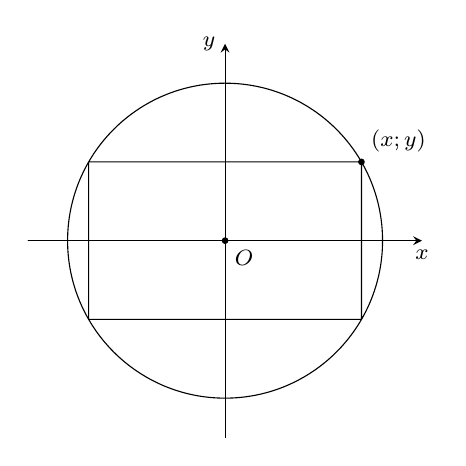
\begin{tikzpicture}[scale=1, font=\footnotesize, line cap=round, line join=round, >=stealth]
\def\r{2}
\path (0,0)coordinate(O)+(30:\r)coordinate(A)+(150:\r)coordinate(B)+(210:\r)coordinate(C)+(-30:\r)coordinate(D);
\draw[->] (-\r-.5,0)--(\r+.5,0)node[below]{$x$};
\draw[->] (0,-\r-.5)--(0,\r+.5)node[left]{$y$};
\draw (O)circle(\r cm) (A)--(B)--(C)--(D)--cycle;
\draw[fill=black] (0,0)node[below right]{$O$}circle(1pt) (A)node[above right]{$(x;y)$}circle(1pt);
\end{tikzpicture}
}
\noindent
Ta có $S(0) = 0$; $S(4) = 0$; $S(2\sqrt{2}) = 32$.\\
Vậy cửa sổ hình chữ nhật lớn nhất nội tiếp đường tròn có bán kính $4$ sẽ là hình vuông với diện tích $32$, chiều dài và chiều rộng bằng $2\sqrt{2} \cdot 2 = 4\sqrt{2}$ (từ $2x$ và $2y$ với $x=y=2\sqrt{2}$).
}
\end{ex}
\TL
\begin{ex}%[0D8H3-2]%[Dự án tex đề CKII - Đợt 15]%[Đình Trí]
Tìm hệ số chứa $ x^4 $ trong khai triển $ (2x-1)^5 $.
\loigiai
{
Ta có
\begin{eqnarray*}
(2x-1)^5 &=&\mathrm{C}_5^0(2x)^5-\mathrm{C}_5^1(2x)^4+\mathrm{C}_5^2(2x)^3-\mathrm{C}_5^3(2x)^2+\mathrm{C}_5^4(2x)-\mathrm{C}_5^5\\
&=& 32x^5-80x^4+80x^3-40x^2+10x-1.
\end{eqnarray*}
Dựa vào khai triển suy ra hệ số chứa $ x^4 $ là $ -80 $.
}
\end{ex}

\begin{ex}%[0D8V2-4]
Một đội thanh niên tình nguyện có $15$ người gồm $12$ nam và $3$ nữ. Hỏi có bao nhiêu cách phân công đội thanh niên tình nguyện đó về giúp đỡ $3$ tỉnh miền núi, sao cho mỗi tỉnh có $4$ nam và $1$ nữ?
\loigiai{
Ta có $\mathrm{C}_3^1\cdot\mathrm{C}_{12}^4$ cách phân công các thanh niên về tỉnh thứ nhất.\\
Với mỗi cách này thì có $\mathrm{C}_2^1 \cdot \mathrm{C}_8^4$ cách phân công số thanh niên còn lại về tỉnh thứ hai.\\
Với mỗi cách phân công trên thì có $\mathrm{C}_1^1\cdot\mathrm{C}_{4}^4$ cách phân công số thanh niên còn lại về tỉnh thứ ba.\\
Do đó, ta có $\mathrm{C}_3^1\cdot\mathrm{C}_{12}^4\cdot\mathrm{C}_2^1\cdot\mathrm{C}_{8}^4\cdot\mathrm{C}_1^1\cdot\mathrm{C}_{4}^4=207900$ cách phân công thỏa mãn đề bài.\\
Gọi số cần lập có dạng $abc$.\\
Chọn $c$ với $c \in\{4;6;8\}$ có $3$ cách.\\
Chọn $\overline{ab}$ có $\mathrm{A}_5^2$ cách.\\
Theo quy tắc nhân, ta có $3 \cdot \mathrm{A}_5^2=60$ số tự nhiên thỏa mãn.
}
\end{ex}

\begin{ex}%[0H9V4-5]%[Dự án đề kiểm tra Toán 10 HK2 NH23-24-BCTuan]%[THPT Nguyễn Thị Minh Khai-TPHCM]
Cho đường tròn $(C)\colon x^2+(y-1)^2=1$ và $A(-2;0)$, $B(2;0)$. Tìm tọa độ điểm $M$ thuộc $(C)$ sao cho $MA+MB$ lớn nhất.
\loigiai{
Dễ thấy đường tròn $(C)$ đi qua $O(0;0)$.\\
Giả sử điểm $M(x;y)$.\\
Ta có
\[MA+MB\le \sqrt{2\left(MA^2+MB^2\right)}=\sqrt{2\left[(x+2)^2+y^2+(x-2)^2+y^2\right]}=\sqrt{4\left(x^2+y^2+4\right)}.\]
\immini
{
Mà $x^2+y^2=MO^2\le (MI+IO)^2=4$.\\
Vậy $MA+MB\le \sqrt{4(4+4)}=4\sqrt{2}$.\\
Dấu bằng xảy ra khi $\heva{& MA=MB \\ & MO=2}\Rightarrow M(0;2)$.
}
{
\begin{tikzpicture}[scale=1,>=stealth, font=\footnotesize, line join=round, line cap=round]
\def\a{-1} \def\b{2} \def\c{2} % Hệ số
\def\xmin{-2.5} \def\xmax{2.5}
\def\ymin{-1} \def\ymax{3}
\draw[->] (\xmin,0)--(\xmax,0) node [below]{$x$};
\draw[->] (0,\ymin)--(0,\ymax) node [left]{$y$};
\node at (0,0) [below left]{$O$};
\clip (\xmin+0.1,\ymin+0.1) rectangle (\xmax-0.1,\ymax-0.1);
\path (-2,0) coordinate (A) (2,0) coordinate (B) (0,1) coordinate (I) ($(I)+(60:1)$) coordinate (M);
\draw (I) circle (1cm);
\draw (M)--(I) (M)--(0,0) (M)--(A) (M)--(B);
\foreach \d/\g in {A/-90,B/-90,I/180,M/70}
\draw[fill=black] (\d) circle (1pt) +(\g:0.3) node{$\d$};
\end{tikzpicture}
}
}
\end{ex}

>>>>>>> 33890a9ce1cfbd3079ed36a93e836cf3ef1fde30
